% @author Arian Helberg

\chapter{Implementierung}
Zur Umsetzung der vorgestellten Konzepte wird im Folgenden auf Softwarepakete, Technologien, Datenspeicherung,
Benutzerinteraktion und Arbeitsablauf der erstellten Software eingegangen.
Darüber hinaus wird ein Überblick über Quellcode und einige Implementierungsentscheidungen gegeben.
Auf Implementierungsdetails zur Nutzung der vorgestellten Technologien wird nicht im Detail eingegangen.
Quellcode wird im Wesentlichen gezeigt und anhand von Zeilenangaben (z.B. \textbf{5}) erläutert.
Softwareumgebungsspezifische Implementierungsdetails werden unter Angabe von drei Punkten (\ldots) weggelassen.

\section{Projektstruktur}
Das Softwareprojekt ist nach der Gradle-Source-Code-Konvention organisiert.
Das gesamte Programm befindet sich im Ordner Generator, der obligatorische Gradle-Dateien und den
Source-Ordner enthält.
Sowohl die Quelldateien, also auch die Testdateien sind der Paketstruktur \textbf{de.haw} untergeordnet.
Die folgende Tabelle gibt einen Überblick über grundlegende Pakete und deren Funktion.

\begin{figure}[H]
    \centering
    \begin{tikzpicture}
        \draw[color=black!60!white]
        \FTdir(\FTroot,root,Generator){
            ++(0,-0.2em)
            \FTdir(root,src,src){
                ++(0,-0.2em)
                \FTdir(src,main,main){
                    ++(0,-0.2em)
                    \FTdir(main,java,java) {
                        ++(0,-0.2em)
                        \FTdir(java,de,de) {
                            ++(0,-0.2em)
                            \FTdir(de,haw,haw) {
                                ++(0,-0.5em)
                                \FTdir(haw,gui,gui) {
                                    ++(0,-0.5em)
                                    \FTdir(gui,shape,shape) {}
                                    ++(0,-0.5em)
                                    \FTdir(gui,structure,structure) {}
                                    ++(0,-0.5em)
                                    \FTdir(gui,template,template) {}
                                    ++(0,-0.5em)
                                    \FTdir(gui,turtle,turtle) {}
                                }
                                ++(0,-0.5em)
                                \FTdir(haw,lsystem,lsystem) {}
                                ++(0,-0.5em)
                                \FTdir(haw,pipeline,pipeline) {
                                    ++(0,-0.5em)
                                    \FTdir(pipeline,pipe,pipe) {}
                                }
                                ++(0,-0.5em)
                                \FTdir(haw,tool,tool) {}
                                ++(0,-0.5em)
                                \FTdir(haw,tree,tree) {}
                                ++(0,-0.5em)
                                \FTdir(haw,tree,utils) {}
                            }
                        }
                    }
                }

                \FTdir(src,test,test) {
                    \FTdir(test,java,java) {
                        \FTdir(java,de,de)
                    }
                }
            }
        };
    \end{tikzpicture}
    \caption{Softwareprojekt Dateistruktur}
\end{figure}

\begin{figure}[H]
    \centering
    \begin{tabular}{l|l}
        \textbf{Paket} &  \textbf{Funktion} \\ \hline
        \textit{gui} & Visualisierung des Programms \\ \hline
        \textit{lsystem} & L-System-Repräsentation \\ \hline
        \textit{pipeline} & Umsetzung des Pipeline-Design-Patterns \\ \hline
        \textit{tool} & Methodiken und Algorithmen \\ \hline
        \textit{tree} & Komponenten der Baumstruktur \\ \hline
        \textit{utils} & Hilfskomponenten
    \end{tabular}
    \caption{Softwarepakete mit zugehörigen Funktionen}
\end{figure}

\section{Technologien}
Zur Umsetzung des Softwarepojektes wird eine Java-Anwendung für die Java-Laufzeitumgebung entwickelt.
Sie liegt in der Distribution \textbf{Amazon Corretto} in der Version 11.0.3\_7 vor.
Grafische Oberflächen werden mit der JavaFX-Spezifikation von Oracle in der Version 11.0.2 umgesetzt.
Zur Automatisierung von Abhängigkeits- und Buildmanagement wird Gradle (Version 6.7) verwendet.
Eine Testumgebung, eine Vektorbibliothek, eine Tupelrepräsentation und eine Erweiterung zur mathematischen
Standartbibliothek werden über Abhängigkeiten vom Gradle-Framework im Build-Prozess geladen und zur Verfügung
gestellt.\\
Um den test-driven Implementierungsansatz umzusetzen wird JUnit 5 Jupiter als Testumgebung genutzt.
Sie setzt sich aus einem Programmierschema und einem Erweiterungsmodell zusammen.
Das Jupiter-Projekt liefert zudem die Laufzeitumgebung für Softwaretests.
Googles Guava liefert eine Bibliothek mit mathematischen Funktionen.
Sie wird benötigt, um eine praktikable Lösung zu Mengenmanipulation nutzen zu können (Bsp. Erstellen
von Kombinationspaaren einer Menge).
Ausschließlich JavaFX wird außerhalb des Projektes installiert und als Modul im Start-Skript des Programmes
hinzugefügt.
\\~\\
Weitere Systeme zur Erstellung des Softwareprojektes sind:
\begin{itemize}
    \item Versionierung via Git,
    \item Dot zur Visualisierung von Graphen und
    \item PlantUML zur Generierung von UML-Diagrammen
\end{itemize}

\newpage

\section{Konzeptumsetzung}

Das Skript \texttt{Generator.bat}, das zum Starten der Anwendung innerhalb eines Windows-Betriebssystems genutzt werden kann,
fügt dem Programm alle externen Module hinzu, die während der Laufzeit genutzt werden, und führt die angegebene jar-Datei aus:
\begin{figure}[H]
    \centering
    \begin{csource}
    java --module-path .\javafx-sdk-11.0.2\lib --add-modules javafx.controls,javafx.fxml,javafx.graphics -jar Generator-1.0.jar
    pause
    \end{csource}
    \caption{Startskript Generator.bat}
\end{figure}

Beim Start der Anwendung findet der Benutzer die grafische Oberfläche vor.
\begin{figure}[H]
    \centering
    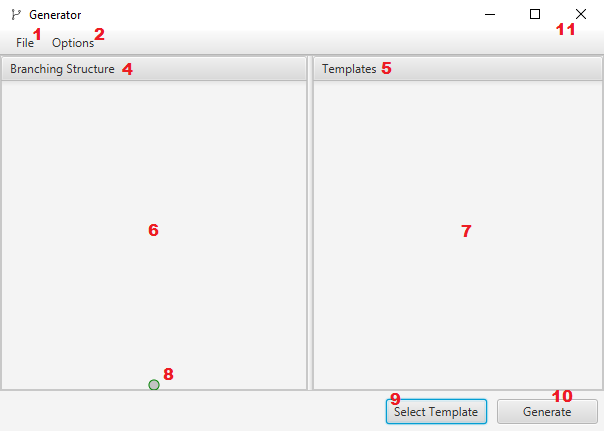
\includegraphics[width=14cm]{../images/UI_numbers1.png}
    \caption{Programm nach Ausführung des Start-Skripts}
\end{figure}
Der Menüeintrag \textbf{1} bietet Funktionen zum Öffnen des Dateipfades und zum Laden der angelegten Templates-Datei.
\textbf{2} dient zur Konfiguration der Umgebungsparameter für die Anzahl Iterationen der Ausführung
und die Anzahl an Ähnlichkeitsstrukturen, die aus dem resultierenden L-System abgeleitet werden können.
Die Gewichtungsparameter der vorgestellten Algorithmen können ebenfalls hier eingestellt werden.
Die Strukturen \textbf{4} und \textbf{5} gliedern das Programm in die Ansicht der Verzweiungsstruktur (\textbf{6}), die vom Benutzer
angelegt wird, die Übersicht zur Auswahl eines Templates (\textbf{7}) und eine Sicht zur Setzung von Transformationsparametern (\textbf{7}).
Der Kreis \textbf{8} stellt einen Anker dar, an welchen eine Template-Instanz angehängt werden kann.
Sowohl über einen Doppelklick, also auch über einen Button (\textbf{9}) kann ein Template aus der Tempalte-Liste (\textbf{7})
ausgewählt werden.
Ist die Verzweigungsstruktur vom Benutzer fertiggestellt, kann die Synthese zur Erstellung der Ähnlichkeitsabbildungen
mit \textbf{10} erfolgen.
Wird der Generieren-Button ohne eine Basisstruktur gedrückt, lässt sich das Beispiel aus
dieser Arbeit erzeugen (ohne visualisierung der Basisstruktur).
\textbf{11} schließt die Anwendung.

\subsection*{Templates}
Eine Datei \textit{template.txt} wird im selben Verzeichnis wie die ausführbare jar-Datei hinerlegt.
Die enthält je eine Template-Zeichenkette pro Zeile, die vom Programm eingelesen und als Template
zur Verfügung gestellt wird.
\begin{figure}[H]
    \centering
    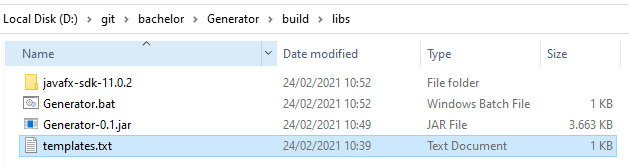
\includegraphics[width=12cm]{../images/templates_file.png}
    \caption{Tempaltes-Datei zum Einlesen der Template-Strukturen}
\end{figure}

\newpage

\subsection*{Visualisierung}
Die grafische Oberfläche liegt als MVC-Pattern in Form des Application State (Model), der XML-basierten FXML-Datei (View)
und dem JavaFX-Controller vor.
Der Arbeitsablauf zur Erstellung der Verzweigungsstruktur kann Schritt für Schritt umgesetzt werden, nachdem die Templates
geladen wurden.
Dies wird an folgendem Beispiel deutlich gemacht.
Die Parameter \textbf{Number of iterations}, \textbf{Number of generations}, \textbf{Rule application ratio} und
\textbf{Merge application ratio} werden auf die Werte \textbf{5}, \textbf{5}, \textbf{0.5} und \textbf{0.5} gesetzt
(Standardeinstellung).
\begin{figure}[H]
    \centering
    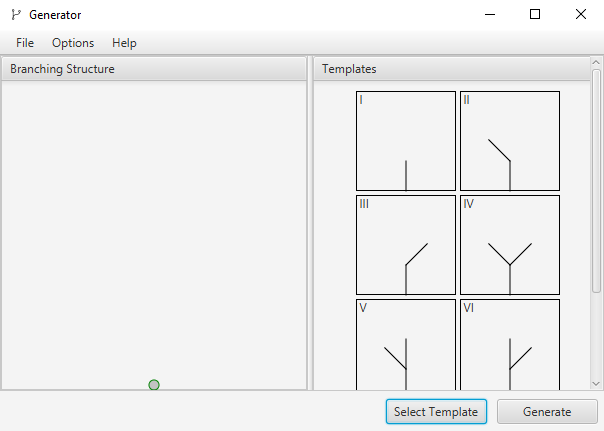
\includegraphics[width=6cm]{../images/UI_templates.png}
    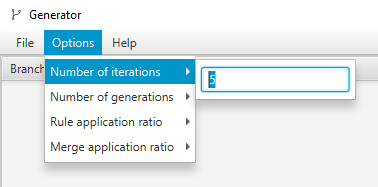
\includegraphics[width=6cm]{../images/UI_parameters.png}
    \caption{Erster Anker ist vorselektiert \& gesetzte Parameter}
\end{figure}

\begin{figure}[H]
    \centering
    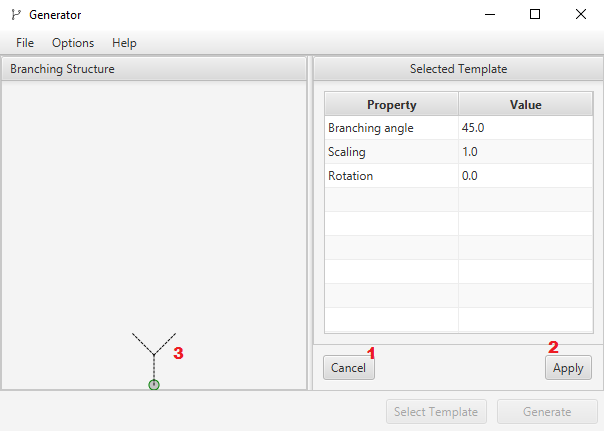
\includegraphics[width=12cm]{../images/UI_template.png}
    \caption{Auswahl des ersten Templates}
\end{figure}

Nachdem ein Template ausgewählt wurde, können die Transformationsparameter gesetzt (Doppelklick) werden und die Auswahl
rückgängig gemacht (\textbf{1}) oder bestätigt (\textbf{2}) werden.
\textbf{3} zeigt einen Entwurf der Tempalte-Instanz, die mit den aktuellen Transformationsparametern angepasst wurde.
Mit der Bestätigung wird die Template-Instanz endgültig der Basisstruktur hinzugefügt und der Benutzer gelangt wieder
in die Übersich der zur Verfügung stehenden Templates.
\begin{figure}[H]
    \centering
    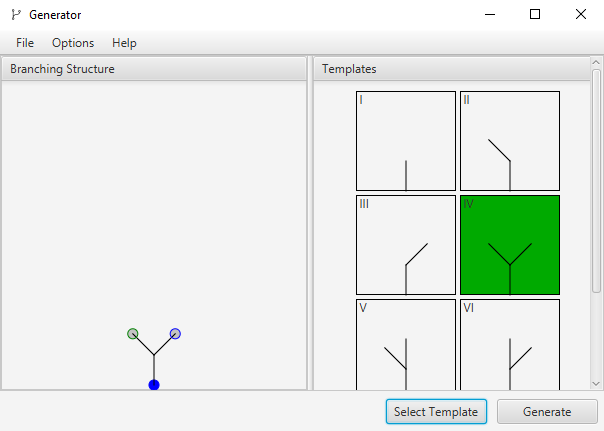
\includegraphics[width=12cm]{../images/UI_applied.png}
    \caption{Der Verzweigungsstruktur hinzugefügte Template-Instanz}
\end{figure}

Dieser Vorgang wiederholt sich, bis der Benutzer die Struktur fertiggestellt hat.
\begin{figure}[H]
    \centering
    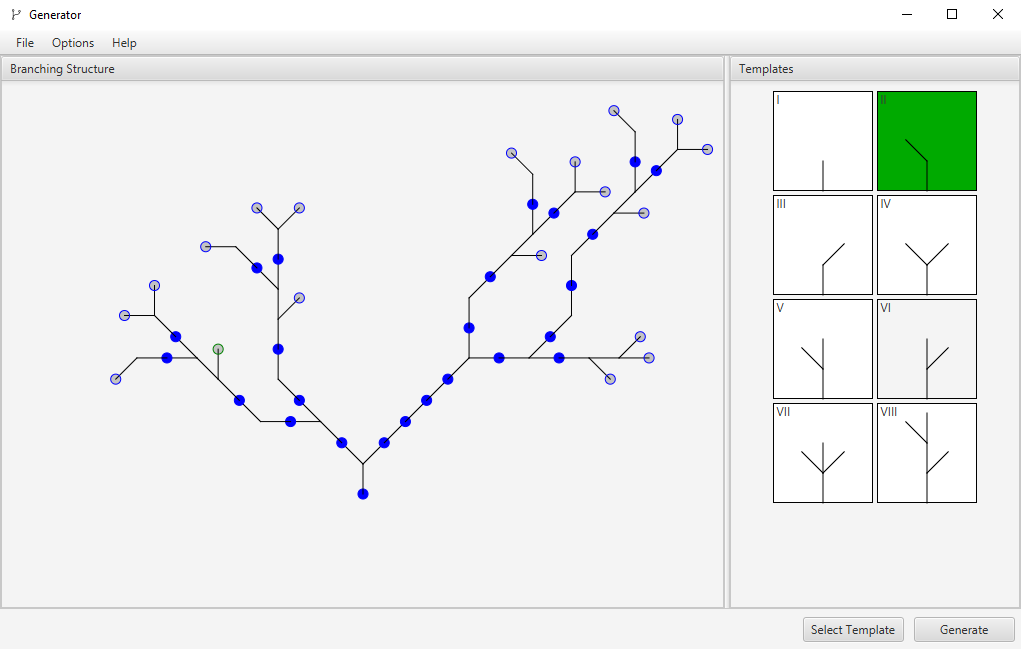
\includegraphics[width=13cm]{../images/UI_finished.png}
    \caption{Vom Benutzer fertiggestellte Verzweigungsstruktur}
\end{figure}

Über den \textbf{Generate}-Button kann nun die Synthese gestartet werden.
Es ergeben sich 5 (\textbf{Number of generations}) Ähnlichkeitsstrukturen
(siehe ~\ref{resulting_structures})

\subsection*{Baumtopologie}
Um eine interne Baumtopologie aufzubauen wird die Klasse \texttt{TreeNode} verwendet, um eine iterierbare Baumstruktur
aufzubauen:

\newpage

\begin{lstlisting}[
    basicstyle=\footnotesize,
    commentstyle=\color{comment},
    keywordstyle=\color{keyword},
    language=Java,
    caption=Klasse TreeNode zur Erstellung einer Baumstruktur,
    frame=tB,
    numberstyle=\color{gray}
]
/**
 * Iterable tree node structure containing a payload and children
 * as tree nodes. Every node represents a whole tree
 */
public class TreeNode<T> implements Iterable<TreeNode<T>> {
    private T data;// Payload
    protected List<TreeNode<T>> children;// Child nodes
    ...
    @Override
    public Iterator<TreeNode<T>> iterator() {
        return new TreeNodeIterator<>(this);
    }
    ...
}
\end{lstlisting}

\texttt{TreeNode} implementiert die \texttt{Iterable}-Schnittstelle, was ein Überladen der \texttt{iterator}-Funktion möglich
macht.
Sie stellt einen Iterator des Baumes zur Verfügung.
Dieser Iterator (\texttt{TreeNodeIterator}) implementiert die \texttt{Iterator}-Schnittstelle und definiert so die Funktionen
\texttt{hasNext} und \texttt{next}.

\begin{lstlisting}[
    basicstyle=\footnotesize,
    commentstyle=\color{comment},
    keywordstyle=\color{keyword},
    language=Java,
    caption=Klasse TreeNodeIterator als Iterator für die Baumstruktur,
    frame=tB,
    numberstyle=\color{gray}
]
/**
 * Tree node iterator for iterating nodes of a tree
 * @param <T> Payload of the tree nodes
 */
public class TreeNodeIterator<T> implements Iterator<TreeNode<T>>{
    ...
    @Override
    public boolean hasNext() {
        return !queue.isEmpty();
    }

    @Override
    public TreeNode<T> next() {
        if (queue.isEmpty()) return null;
        var node = queue.pop();
        queue.addAll(node.getChildren());
        return node;
    }
}
\end{lstlisting}
Die Funktion \texttt{next} zeigt, wie eine Iteration des Baumes als Breitensuch e implementiert ist.
Diese wird beim Inferieren eines L-Systems aus der Baumstruktur benötigt.
Das folgende Beispiel zeigt eine erstellte Baumstruktur (links) und deren erstellte Baumtopologie (rechts).
\begin{figure}[H]
    \centering
    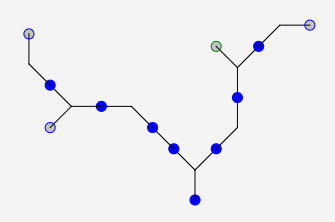
\includegraphics[width=8cm]{../images/graph_tree.png}
    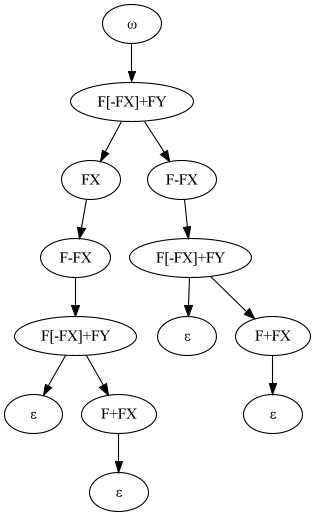
\includegraphics[width=5cm]{../images/tree_graph.png}
    \caption{Verzweigungsstruktur \& zugehörige Baumstruktur}
\end{figure}

\subsection*{Prozesspipeline}
Das angewendete Pipeline-Design-Pattern zur Umsetzung der Inferrierung, Komprimierung und Generalisierung von L-Systemem,
sowie der Verteilung von Transformationsparametern bei deren Ausführung, setzt sich aus der \texttt{Pipeline}-Klasse und
dem \texttt{Pipe}-Interface zusammen.

\newpage

\begin{lstlisting}[
    basicstyle=\footnotesize,
    commentstyle=\color{comment},
    keywordstyle=\color{keyword},
    language=Java,
    caption=Pipeline Klasse zur Organisation von Prozessen,
    frame=tB,
    numberstyle=\color{gray}
]
/**
 * Pipeline class to set up a pipeline design pattern.
 * Classes implementing the Pipe interface can be executed in a specific
 * order while updating a pipeline context
 * @param <IN> Pipeline input type
 * @param <OUT> Pipeline output type
 */
public class Pipeline<IN, OUT> {
    private final Pipe<IN, OUT> current;

    public Pipeline(Pipe<IN, OUT> pipe) {
        current = pipe;
    }

    public <NewO> Pipeline<IN, NewO> pipe(Pipe<OUT, NewO> next) {
        return new Pipeline<>(input -> next.process(current.process(input)));
    }

    public OUT execute(IN input) {
        return current.process(input);
    }
}
\end{lstlisting}

\begin{lstlisting}[
    basicstyle=\footnotesize,
    commentstyle=\color{comment},
    keywordstyle=\color{keyword},
    language=Java,
    caption=Pipe Interface als Vorlage zur Erstellung eines Teilprozesses einer Pipeline,
    frame=tB,
    numberstyle=\color{gray}
]
/**
 * Pipe class as a process to be part of a pipeline
 * @param <IN> Pipe input type
 * @param <OUT> Pipe output type
 */
public interface Pipe<IN, OUT> {
    OUT process(IN input);
}
\end{lstlisting}

Die eigentliche Umsetzung der Prozesspipeline zur Synthese der Verzweigungsstrukturen wird wie folgt implementiert.
Hierbei implementieren die Klassen \texttt{InfererPipe}, \texttt{CompressorPipe}, \texttt{GeneralizerPipe} und
\texttt{EstimatorPipe} das \texttt{Pipe}-Interface und geben die Reihenfolge des Prozesses an.
Das \texttt{ctx}-Objekt wird als Kontextobjekt in die Pipeline gegeben und bei jedem Prozessschritt angepasst.

\newpage

\begin{lstlisting}[
    basicstyle=\footnotesize,
    commentstyle=\color{comment},
    keywordstyle=\color{keyword},
    language=Java,
    caption=Erstellen des Pipeline Kontextes,
    frame=tB,
    numberstyle=\color{gray}
]
...
var ctx = new PipelineContext();
...
// Execute pipeline
var result = new Pipeline<>(new InfererPipe())
        .pipe(new CompressorPipe())
        .pipe(new GeneralizerPipe())
        .pipe(new EstimatorPipe())
        .execute(ctx);
...
\end{lstlisting}

\subsection*{Inferrierung eines L-Systems aus einer Baumstruktur}
Die Inferrierung des L-Systems findet in der Klasse \texttt{Inferer} statt, die in der \texttt{InfererPipe}-Klasse erstellt wird.
Sie nimmt die Baumstruktur entgegegen und stellt eine Funktion \texttt{infer} zum Inferieren des L-Systems zur Verfügung.
\begin{lstlisting}[
    basicstyle=\footnotesize,
    commentstyle=\color{comment},
    keywordstyle=\color{keyword},
    language=Java,
    numberstyle=\color{gray},
    caption=Inferer Klasse zur Inferrierung eines L-Systems aus einer Baumstruktur,
    frame=tB,
    numbers = left
]
/**
 * Inferer to infer a L-System out of a tree-like data structure
 */
public class Inferer {
    ...
    public Inferer(TreeNode<TemplateInstance> tree) {
        //// Initializing
        lSystem = new LSystem();
        // M = {F, S}
        lSystem.addModule("F","S");
        // w = S
        lSystem.setAxiom("S");
        // R <- { alpha: S -> A }
        var alpha = new ProductionRule("S", "A");
        lSystem.addProductionRule(alpha);
        // beta = next node
        beta = iterator.next();
        // M <- gamma in { A, B, ..., Z }, with gamma not in M
        gamma = lSystem.addModuleNotPresentInAlphabet();
    }
    ...
}
\end{lstlisting}

Das erstellte L-System (\textbf{8}) wird während des Inferierens aktualisiert und am Schluss als Ergebnis zurückgegeben.
Dann werden die initialen Symbole $F$ und $S$ hinzugefügt und das Axiom auf $S$ gesetzt (\textbf{10-12}).
Die initiale Produktionsregel $\alpha: S \rightarrow A$ wird erstellt und der Produktionsregelmenge beigefügt (\textbf{14-15}).
Es wird der erste zu untersuchende Knoten des Baumen über seinen Iterator zurückgegeben und als $\beta$ gesetzt (\textbf{17}).
Am Ende der Initialisierung fügt die Methode \texttt{addModuleNotPresentInAlphabet} dem Alphabet ein neues Symbol (\texttt{gamma}) hinzu,
das dort nicht vorhanden ist (\textbf{19}).
Dies geschieht nach lexikografischer Reihenfolge.

Nach der Erstellung des \texttt{Inferer}-Objektes kann in der zugehörigen Pipe \texttt{InfererPipe} das L-System inferriert
werden
\begin{lstlisting}[
    basicstyle=\footnotesize,
    breaklines = true,
    commentstyle=\color{comment},
    keywordstyle=\color{keyword},
    language=Java,
    numberstyle=\color{gray},
    numbers = left,
    caption=InfererPipe Klasse als Teilprozess der Pipeline,
    frame=tB,
    postbreak=\mbox{\textcolor{gray}{\ArrowBoldDownRight}\space}
]
/**
 * Pipe for executing the infer algorithm.
 * It takes the pipeline context, set it accordingly to the result
 * and returns it to the next pipe
 */
public class InfererPipe implements Pipe<PipelineContext, PipelineContext>, Logging {
    ...
    @Override
    public PipelineContext process(PipelineContext input) {
    ...
    // Update pipeline context
    input.lSystem = new Inferer(input.tree).infer();
    ...
    }
}
\end{lstlisting}

Die \texttt{infer}-Methode extrahiert die Zeichenkette (Wort) des im aktuellen Baumknoten gespeicherten Template-Instanz
(\textbf{9}) und speichert sie zur Bearbeitung in \texttt{delta}.
Delta wird nach Verzweigungsvariablen durchsucht (\textbf{11-14}) und diese dann durch ein neues Symbol,
das dem Alphabet hinzugefügt wird (\textbf{18}), ersetzt (\textbf{20}).
Eine neue Produktionsregel, die \texttt{gamma} auf das veränderte Wort abbildet, wird dem L-System beigefügt (\textbf{24}).
\textbf{31-35} sucht nach Symbolen im Alphabet, die noch kein Ziel einer Produktionsregel sind und hält diese in der
Variablen \texttt{gamma}.
Wird kein solches Symbol gefunden, terminiert die \texttt{infer}-Methode und damit der Algorithmus (\textbf{44}).
Der aktuelle Knoten wird durch den Iterator der Baumstruktur mit dem nächsten Knoten nach Breitensuche ersetzt (\textbf{46}).
Zum Schluss wird das inferrierte L-System zurückgegeben (\textbf{48}).

Für die Implementierung des Inferrierungsalgorithmus siehe \ref{infer}

Die übrigen Prozessschritte sind ähnlich aufgebaut.
Auch die Klassen \texttt{Compressor}, \texttt{Generalizer} und \texttt{Estimator} implementieren eine Funktion zum Ausführer
der jeweiligen Algorithmen, während die Initialisierung im Konstruktor ausgeführt wird.
Dabei wird die Implementierung der Algorithmen eng an der Konzeptionierung gehalten (siehe Kapitel ~\ref{algo}).
Alle weiteren Klassen der Basisalgorithmen werden im Folgenden gezeigt und Spezialfälle erläutert.

\subsection*{Komprimierung des L-Systems}
\begin{lstlisting}[
    basicstyle=\footnotesize,
    breaklines = true,
    commentstyle=\color{comment},
    keywordstyle=\color{keyword},
    language=Java,
    numberstyle=\color{gray},
    numbers = left,
    caption=Klasse Compressor zur Komprimierung eines L-Systems,
    frame=tB,
    postbreak=\mbox{\textcolor{gray}{\ArrowBoldDownRight}\space}
]
/**
 * Compressor class for compressing a L-System.
 * The algorithms searches for identical, maximal subtrees
 * and replaces them with combined instances
 */
public class Compressor {
    ...
    public Compressor(TreeNode<TemplateInstance> tree, LSystem lSystem, float wL, Random randomizer) {
        //// Initializing
        this.tree = tree.copy();
        this.LPlus = lSystem;
        // L = ∅
        this.L = new LSystem();
        // wl ∈ [0, 1]
        weighting = wL;
        this.randomizer = randomizer;
    }
    ...
}
\end{lstlisting}

Für den Komprimierungsalgorithmus siehe~\ref{compress}

\newpage

\begin{lstlisting}[
    basicstyle=\footnotesize,
    breaklines = true,
    commentstyle=\color{comment},
    keywordstyle=\color{keyword},
    language=Java,
    linewidth=15cm,
    numberstyle=\color{gray},
    numbers = left,
    caption=Algorithmus zum Finden eines maximalen Unterbaums,
    frame=tB,
    postbreak=\mbox{\textcolor{gray}{\ArrowBoldDownRight}\space}
]
/**
 * Search and for maximum sub-tree that appears more than one time
 * in the tree and return it
 * @param tree Tree to be searched
 * @return Maximum sub-tree
 */
private TreeNode<TemplateInstance> FindMaximumSubTree(TreeNode<TemplateInstance> tree) {
    var globalIterator = tree.iterator();
    globalIterator.next();
    // Iterate
    while (globalIterator.hasNext()) {
        var globalNode = globalIterator.next();
        var localIterator = tree.iterator();
        var l = localIterator.next();
        while (l != globalNode) l = localIterator.next();
        while (localIterator.hasNext()) {
            var localNode = localIterator.next();
            if (!globalNode.isLeaf()) {
                // Check for equality / check for appearance > 1 in the tree
                if (Trees.compare(globalNode, localNode)) return globalNode;
            }
        }
    }
    return null;
}
\end{lstlisting}

\newpage

\begin{lstlisting}[
    basicstyle=\footnotesize,
    breaklines = true,
    commentstyle=\color{comment},
    keywordstyle=\color{keyword},
    language=Java,
    numberstyle=\color{gray},
    numbers = left,
    caption=Algorithmus zum Finden alle Vorkommen eines Unterbaums in einem Baum,
    frame=tB,
    postbreak=\mbox{\textcolor{gray}{\ArrowBoldDownRight}\space}
]
/**
 * Find all occurrences of a sub-tree in a tree
 * @param subtree Sub-tree to be searched for
 * @param tree Tree that contains the sub-tree
 * @return List of sub-trees
 */
private List<TreeNode<TemplateInstance>> getOccurrences(TreeNode<TemplateInstance> subtree, TreeNode<TemplateInstance> tree) {
    var iterator = tree.iterator();
    iterator.next();
    // Store occurrences
    var occurrences = new ArrayList<TreeNode<TemplateInstance>>();
    // Iterate through the tree
    while (iterator.hasNext()) {
        var node = iterator.next();
        if (Trees.compare(node, subtree)) {
            // Subtree to be replaced found
            occurrences.add(node);
        }
    }
    return occurrences;
}
\end{lstlisting}
\begin{lstlisting}[
    basicstyle=\footnotesize,
    breaklines = true,
    commentstyle=\color{comment},
    keywordstyle=\color{keyword},
    language=Java,
    numberstyle=\color{gray},
    numbers = left,
    caption=Funktion zur Berechnung der Kosten eines L-Systems,
    frame=tB,
    postbreak=\mbox{\textcolor{gray}{\ArrowBoldDownRight}\space}
]
/**
 * Return the costs of a L-System combining the length of the alphabet
 * and the number of rule applications of the production rules
 * @param lSystem L-System to be measured
 * @return Costs of the L-System
 */
private float Ci(LSystem lSystem) {
    var costs = 0;
    for (var rule : lSystem.getProductionRules()) {
        costs += weighting * rule.getRhs().length() + (1 - weighting) * countRuleApplications(lSystem, rule.getLhs());
    }
    return costs;
}
\end{lstlisting}

\newpage

\begin{lstlisting}[
    basicstyle=\footnotesize,
    breaklines = true,
    commentstyle=\color{comment},
    keywordstyle=\color{keyword},
    language=Java,
    numberstyle=\color{gray},
    numbers = left,
    caption=Funktion zur Ermittlung der Anzahl Anwendung einer Produktionsregel,
    frame=tB,
    postbreak=\mbox{\textcolor{gray}{\ArrowBoldDownRight}\space}
]
/**
 * Counts the production rule applications in a string and returns it
 * @param lSystem L-System to be searched
 * @param lhs LHS of a production rule
 * @return Number of production rule applications
 */
private int countRuleApplications(LSystem lSystem, String lhs) {
    int occurrences = 0;
    var pattern = Pattern.compile(lhs);
    // Check axiom
    var axiomMatcher = pattern.matcher(lSystem.getAxiom());
    while (axiomMatcher.find()) occurrences++;
    // Check production rules
    var ruleMatcher = pattern.matcher(lSystem.getProductionRules().stream()
            .map(ProductionRule::getRhs).collect(Collectors.joining()));
    while (ruleMatcher.find()) occurrences++;
    return occurrences;
}
\end{lstlisting}

\subsection*{Generalisierung des L-Systems}
\begin{lstlisting}[
    basicstyle=\footnotesize,
    breaklines = true,
    commentstyle=\color{comment},
    keywordstyle=\color{keyword},
    language=Java,
    numberstyle=\color{gray},
    numbers = left,
    caption=Generalizer Klasse zur Generalisierung eines L-Systems,
    frame=tB,
    postbreak=\mbox{\textcolor{gray}{\ArrowBoldDownRight}\space}
]
/**
 * Generalizer class to add non-deterministic rules to an L-System
 */
public class Generalizer {
    ...
    public Generalizer(LSystem lSystem, float w0) {
        //// Initialization
        // Generalized grammar L* = L+ (compact grammar)
        LStar = lSystem.copy();
        // metric weight balancing
        this.w0 = w0;
        // C^old_g = Cg(L∗ + {p∗}, L∗)
        Cg_old = 0;
        // cStar
        cStar = 0;
    }
    ...
}
\end{lstlisting}

Für den Generalisierungsalgorithmus siehe~\ref{generalize}

\begin{lstlisting}[
    basicstyle=\footnotesize,
    breaklines = true,
    commentstyle=\color{comment},
    keywordstyle=\color{keyword},
    language=Java,
    numberstyle=\color{gray},
    numbers = left,
    caption=Kostenfunktion zum Vergleich zweier L-Systeme,
    frame=tB,
    postbreak=\mbox{\textcolor{gray}{\ArrowBoldDownRight}\space}
]
/**
 * Calculates the costs of editing a grammar leveraging the grammar
 * length and the grammar edit distance both weighted with a weight
 * balancing w0 ∈ [0.0, 1.0]
 */
private float Cg(LSystem lStar, LSystem lPlus) {
    return w0 * (L(lStar) - L(lPlus)) + (1 - w0) * Dg(lStar);
}
\end{lstlisting}
\begin{lstlisting}[
    basicstyle=\footnotesize,
    breaklines = true,
    commentstyle=\color{comment},
    keywordstyle=\color{keyword},
    language=Java,
    numberstyle=\color{gray},
    numbers = left,
    caption=Längenfunktion über ein L-System,
    frame=tB,
    postbreak=\mbox{\textcolor{gray}{\ArrowBoldDownRight}\space}
]
/**
 * Measure and return the length of a L-System
 * @param lSystem L-System to be measured
 * @return L-System length
 */
private int L(LSystem lSystem) {
    // Set size of the alphabet M
    var M_size = lSystem.getAlphabet().size();
    // Sum of RHS symbols over all production rules
    var sum_rulesRHSs = lSystem.getProductionRules().stream()
            .map(r -> r.getRhs().length())
            .mapToInt(Integer::intValue)
            .sum();
    return M_size + sum_rulesRHSs;
}
\end{lstlisting}

\newpage

\begin{lstlisting}[
    basicstyle=\footnotesize,
    breaklines = true,
    commentstyle=\color{comment},
    keywordstyle=\color{keyword},
    language=Java,
    linewidth=15cm,
    numberstyle=\color{gray},
    numbers = left,
    caption=Grammar Edit Distance,
    frame=tB,
    postbreak=\mbox{\textcolor{gray}{\ArrowBoldDownRight}\space}
]
/**
 * Grammar edit distance: Overall costs to convert a grammar to another
 * by a set of merging operations M(L+ -> L*)
 */
private float Dg(LSystem lStar) {
    // Grammar edit distance
    var editDistance = 0;
    // Get all multi-module production rules
    var rules = lStar.getProductionRules().stream()
            .filter(rule -> rule.getLhs().length() > 1)
            .collect(Collectors.toList());

    // Go through all merging operations (merging two rules)
    while (!rules.isEmpty()) {
        var operation1 = rules.get(0);
        // Find corresponding rules
        var otherOperations = rules.stream()
                .filter(r -> !r.equals(operation1) && r.getLhs().equals(operation1.getLhs()))
                .collect(Collectors.toList());

        rules.remove(operation1);

        if (!otherOperations.isEmpty()) {
            var iterator = otherOperations.iterator();
            do {
                // Ds(M*_A,M*_B)
                var operation = iterator.next();
                editDistance += Ds(operation1.getRhs(), operation.getRhs());
                rules.remove(operation);
            } while (iterator.hasNext());
        }
    }

    return editDistance;
}
\end{lstlisting}

\newpage

\begin{lstlisting}[
    basicstyle=\footnotesize,
    breaklines = true,
    commentstyle=\color{comment},
    keywordstyle=\color{keyword},
    language=Java,
    numberstyle=\color{gray},
    numbers = left,
    caption=String Edit Distance,
    frame=tB,
    postbreak=\mbox{\textcolor{gray}{\ArrowBoldDownRight}\space}
]
/**
 * Calculate and return the edit distance between two strings
 * @param M_A String A
 * @param M_B String B
 * @return Edit distance between A and B
 */
private float Ds(String M_A, String M_B) {
    return Modules.editDistanceOptimized(M_A, M_B);
}
\end{lstlisting}
\begin{lstlisting}[
    basicstyle=\footnotesize,
    breaklines = true,
    commentstyle=\color{comment},
    keywordstyle=\color{keyword},
    language=Java,
    numberstyle=\color{gray},
    numbers = left,
    caption=Modules Klasse mit Funktion zur Ermittlung der String Edit Distance,
    frame=tB,
    postbreak=\mbox{\textcolor{gray}{\ArrowBoldDownRight}\space}
]
public class Modules {
    ...
    /**
     * Calculate and return the edit distance between two strings
     * Time complexity: O(m*n)
     * Space complexity: O(m)
     * @param str1 String A
     * @param str2 String B
     * @return Edit distance between A and B
     */
    public static int editDistanceOptimized(String str1, String str2) {
        int len1 = str1.length();
        int len2 = str2.length();
        int[][] DP = new int[2][len1 + 1];
        for (int i = 0; i <= len1; i++) DP[0][i] = i;
        for (int i = 1; i <= len2; i++) {
            for (int j = 0; j <= len1; j++) {
                if (j == 0) DP[i % 2][j] = i;
                else if (str1.charAt(j - 1) == str2.charAt(i - 1)) DP[i % 2][j] = DP[(i - 1) % 2][j - 1];
                else DP[i % 2][j] = 1 + Math.min(DP[(i - 1) % 2][j], Math.min(DP[i % 2][j - 1], DP[(i - 1) % 2][j - 1]));
            }
        }
        return DP[len2 % 2][len1];
    }
}
\end{lstlisting}

Der Algorithmus \texttt{editDistanceOptimized} ist aus Praktikabilitätsgründen aus~\cite{editdistance}
entnommen.

\subsection*{Verteilung der Transformationsparameter}
\begin{lstlisting}[
    basicstyle=\footnotesize,
    breaklines = true,
    commentstyle=\color{comment},
    keywordstyle=\color{keyword},
    language=Java,
    numberstyle=\color{gray},
    numbers = left,
    caption=Estimator Klasse zur Erstellung einer Verteilung über Transformaitonsparameter,
    frame=tB,
    postbreak=\mbox{\textcolor{gray}{\ArrowBoldDownRight}\space}
]
/**
 * Estimator class to create a distribution of different
 * transformation parameters
 */
public class Estimator {
    ...
    public Estimator(Random randomizer) {
        /// Initialization
        parameters = new HashMap<>();
        this.randomizer = randomizer;
    }
    ...
}
\end{lstlisting}

Für den Verteilungsalgorithmus siehe~\ref{estimate}

\begin{lstlisting}[
    basicstyle=\footnotesize,
    breaklines = true,
    commentstyle=\color{comment},
    keywordstyle=\color{keyword},
    language=Java,
    numberstyle=\color{gray},
    numbers = left,
    caption=Abrufen eines zufälligen Parameters aus der Verteilung für ein Template,
    frame=tB,
    postbreak=\mbox{\textcolor{gray}{\ArrowBoldDownRight}\space}
]
...
/**
 * Estimate and return a parameter for a given template by name
 * @param parameter Parameter name
 * @param templateID Corresponding template
 * @return Estimated parameter value
 */
public float estimateParameterValueForTemplate(String parameter, int templateID) {
    var entries = parameters.get(parameter).get(templateID);
    return entries.get(randomizer.nextInt(entries.size()));
}
...
\end{lstlisting}

\newpage

\begin{lstlisting}[
    basicstyle=\footnotesize,
    breaklines = true,
    commentstyle=\color{comment},
    caption=test algo,
    frame=tB,
    keywordstyle=\color{keyword},
    language=Java,
    linewidth=15cm,
    numberstyle=\color{gray},
    numbers = left,
    caption=Berechnung des Durchschnitts eines Parameters für ein Template,
    frame=tB,
    postbreak=\mbox{\textcolor{gray}{\ArrowBoldDownRight}\space}
]
...
/**
 * Calculate and return the average value for a parameter for a
 * given template by name
 * @param parameter Parameter name
 * @param templateID Corresponding template
 * @return Averaged parameter value
 */
public float averageParameterValueForTemplate(String parameter, int templateID) {
    var entries = parameters.get(parameter).get(templateID);
    return (float) entries.stream().mapToDouble(v -> v).average().orElse(0);
}
...
\end{lstlisting}